%% V1.0
%% by Gabriel Garcia, gabrcg@gmail.com
%% This is a template for Udacity projects using IEEEtran.cls

%% Be Udacious!

\documentclass[10pt,journal,compsoc]{IEEEtran}

\usepackage[pdftex]{graphicx}    
\usepackage{cite}
\hyphenation{op-tical net-works semi-conduc-tor}
\usepackage{hyperref}
\usepackage{enumerate}


\begin{document}

\title{RTAB-Map SLAM Project}

\author{Pritesh Gudge}

\markboth{Simultaneous Mapping and Localization Project, Robotics Nanodegree Program, Udacity}%
{}
\IEEEtitleabstractindextext{%

\begin{abstract}
The third project in term 2 of the Udacity Robotics Nano Degree program requires students to use ROS and Gazebo along with RTAB-Map, to create a 2D occupancy grid and a 3D octomap of two environments(worlds) - one supplied as a part of the project and the other custom generated. The project aims at performing an application of SLAM techniques in a simulated environment.
The objective is to extend a previous robot creation to upgrade sensors to supply the necessary sensor messages for RTAB-Map. This leverages the laser scanner, IMU/Wheel Encoder but replaces the camera with a RGB-D camera (ie kinect).
Further the ROS project is created with all links connected with appropriate naming and mapping.
The robot is launched and teleoped around the environments to generate a map of the environment. After successfully mapping the supplied environment, a custom generated environment is created and mapped using the same technique.
\end{abstract}

% Note that keywords are not normally used for peerreview papers.
\begin{IEEEkeywords}
Robot, IEEEtran, Udacity, \LaTeX, SLAM.
\end{IEEEkeywords}}


\maketitle
\IEEEdisplaynontitleabstractindextext
\IEEEpeerreviewmaketitle
\section{Introduction}
\label{sec:introduction}

\IEEEPARstart{T}{he} robot model in this project uses a Simultaneous Localisation and Mapping (SLAM) technique called RTAB-Map (Real-Time Appearance-Based Mapping). It is a RGB-D Graph Based SLAM approach that uses incremental appearance based loop closure detection\cite{loopclosure}.
The RTAB-Map ROS wrapper\cite{rosrtabmap} is leveraged with visual representation in real time via rtabmapviz. The resultant map is stored in local database that be later interrogated via rtabmap-databaseViewer\cite{rtabdbviewer}.


%example for inserting image
\begin{figure}[thpb]
      \centering
      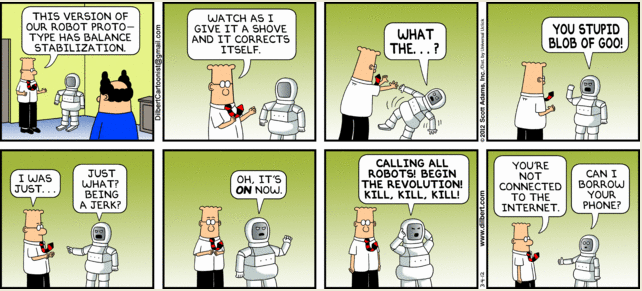
\includegraphics[width=\linewidth]{RobotRevolution5}
      \caption{Robot Revolution.}
      \label{fig:robot1}
\end{figure}

\subsection{Subsection Heading Here}
Subsection text here.

\subsubsection{Subsubsection Heading Here}
Subsubsection text here.

%example for building table
\begin{table}[h]
\caption{Table}
\label{table_example}
\begin{center}
\begin{tabular}{|c||c|}
\hline
One & Two\\
\hline
Three & Four\\
\hline
\end{tabular}
\end{center}
\end{table}



\section{Background}
When a robot encounters a new environment where there is no supplied map, it needs to be able to create this map and localise its pose using it. This combined localisation and mapping process is referred to as SLAM (Simultaneous Localisation and Mapping).

The main mapping algorithms are Occupancy Grid Mapping, Grid-based FastSLAM, Graph-SLAM and RTAB-Map.

\subsection{Occupancy Grid Mapping}
The Occupancy Grid Mapping\cite{occgripmap} is a 2D algorithm where each grid cell is identified as Unknown/Undiscovered Zone, Free Zone or Occupied. This represents a slice of the 3D world.

\subsection{Grid-Based FastSLAM}
The Grid-Based FastSLAM\cite{gridslam} approach combines SLAM (Synchronised Location and Mapping) using a MCL (Monte Carlo Localisation) Algorithm and an Occupancy Grid Mapping. The main advantage of is the MCL particle filter approach but it always assumes there are known landmark positions. Thus it is unable to model an arbitrary environment.

\subsection{Graph SLAM}
Graph-SLAM\cite{graphslam} uses a graph based approach to represent poses, features from the environment, motion constraints (between two poses) and measurement constraints (ties together a feature and a pose). It solves the full SLAM problem, it covers the entire path and map and not the most recent pose.

\subsection{RTAB-Map}
This project uses RTAB-Map\cite{rosrtabmap}, which is a Graph-SLAM approach that uses loop closure with Visual Bag-of-Words\cite{vbow} for optimisation.
The loop closure detection occurs against working memory to constrain the number of images interrogated. Working memory can be transferred and retrieved from long term memory to reduce complexity. The algorithm used for loop closure detection is SURF (Speeded Up Robust Features)\cite{surf}.

The possible outputs of RTAB-Map are 2D occupancy grid map, 3D octomap or a 3D point cloud.

Robots are of varying dimensions inclusive of height. Whilst mapping a 2d environment may show where fixed walls etc are it does not take into account height. A robot, that is propelled on the floor, may be able to navigate under some obstacles but not others eg a chair vs a large table. Hence the need to understand the environment from a 3D perspective.

However building a 3D map is more costly then a 2D map. This is not only in terms of Compute \& Data costs but also in the cost of the sensors required. However, simple sensors such as a single camera may be cheaper but the algorithms required can be more complex.



%example for Bullet point list
\begin{itemize}
\item example 1
\item example 2
\end {itemize}

%example for numbered list
\begin{enumerate}
\item example 1
\item example 2
\end{enumerate}

\section{Simulations}

\subsection{Robot Model Configuration}
The robot model used was based on the udacity\_bot created in the previous project as the  robot model (which had a rectangular base with differential drive controller for the left and right wheels). The camera was removed and replaced with a kinect leveraging the \emph{openni\_camera} ros package with the gazebo controller \emph{Openni Kinect}.
No changes were made to the hokuyo laser range finder.
An additional joint was added to rotate the kinect data 180 degrees. It was positioned on the front of the robot so as to not interfere with the laser range finder.
The bot configuration files can be found under the urdf directory.
Visualization of the frames follows is show in the figure \ref{fig:frame}.

\begin{figure}[thpb]
      \centering
      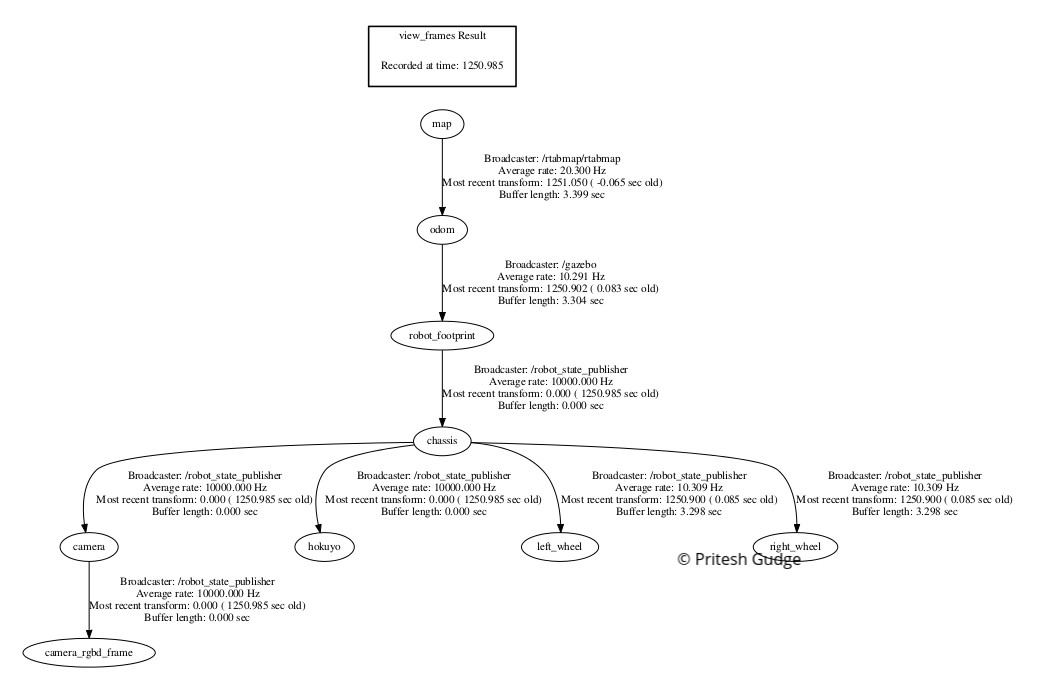
\includegraphics[width=\linewidth]{images/tfframe}
      \caption{TF Frame}
      \label{fig:frame}
\end{figure}

% Robot Models
\subsection{Worlds}
Two worlds were created in gazebo - one supplied as kitchen\_dining.world (Fig. \ref{fig:kitchenworld})and the other customised cafekitchen.world (Fig. \ref{fig:customworld})
\begin{figure}[thpb]
      \centering
      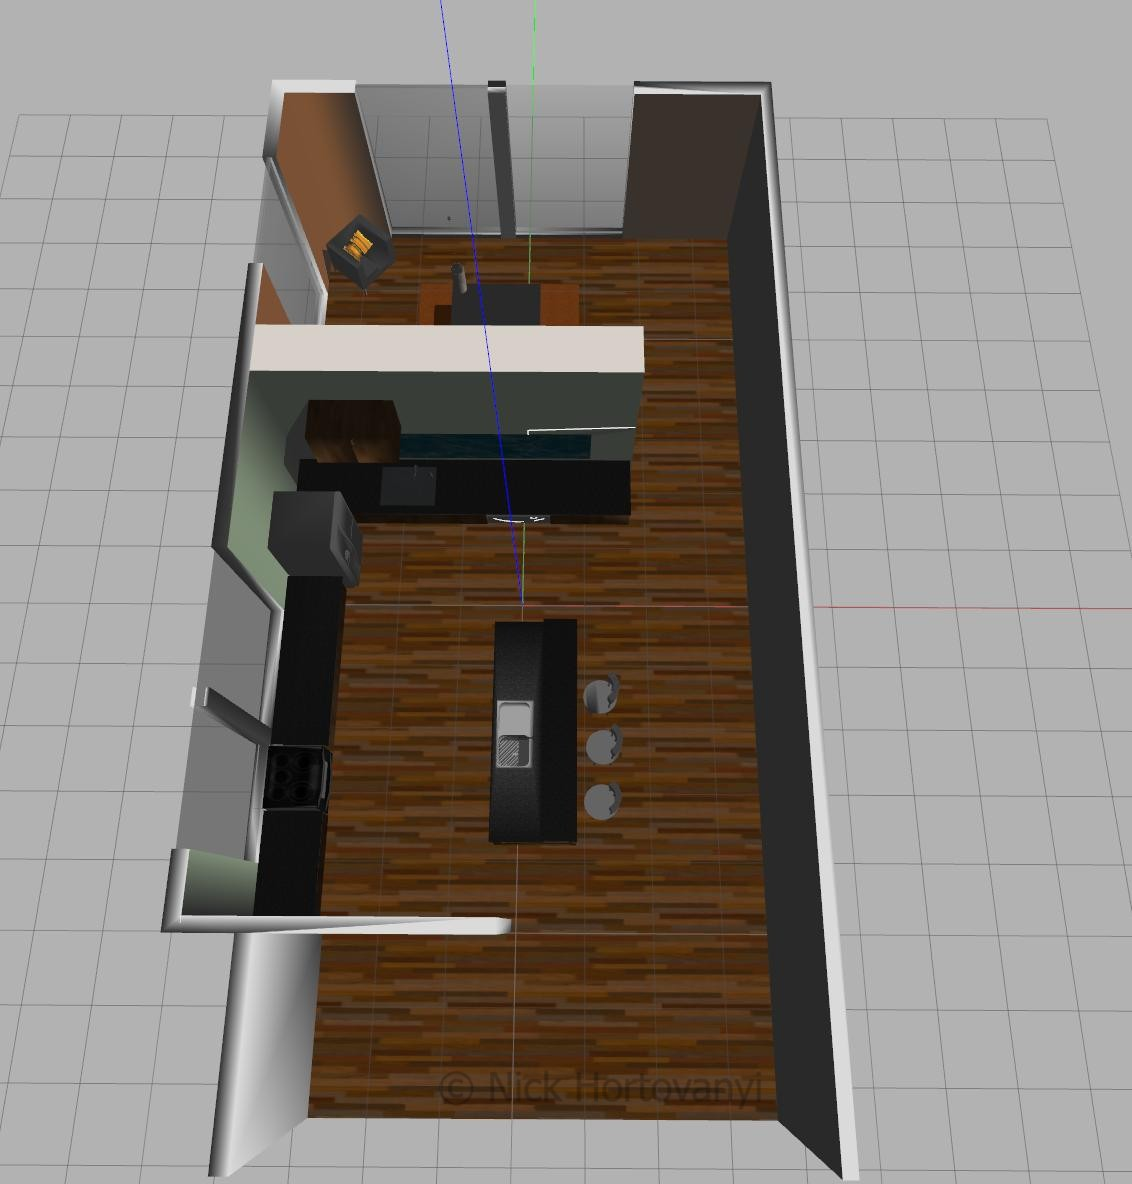
\includegraphics[width=\linewidth]{images/gazebokitchenworld}
      \caption{Kitchen World}
      \label{fig:kitchenworld}
\end{figure}

\begin{figure}[thpb]
      \centering
      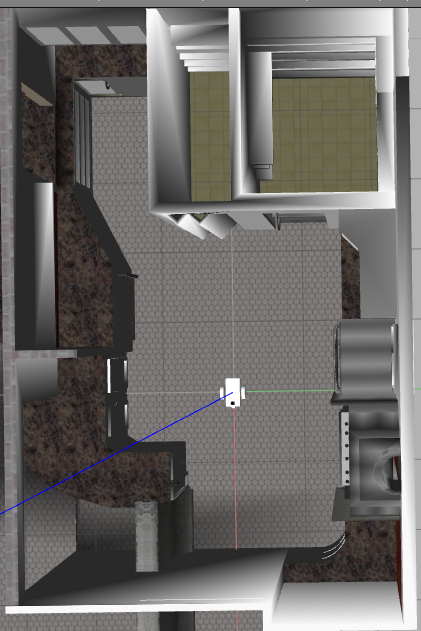
\includegraphics[width=\linewidth]{images/cafekitchen}
      \caption{Custom World}
      \label{fig:customworld}
\end{figure}

\subsubsection{Parameters}
The Kitchen World model was mapped with RtabMap features Kp/MaxFeatures 400 and Vis/MinInliers at 15.




\section{Results}

\subsection{Kitchen World}
The kitchen world 2D and 3D maps are shown in figure\ref{fig:kitchen2d} and figure \ref{fig:kitchen3d} respectively. In the 2D Map and the 3D map the general layout of the kitchen and the furniture structures are visible. 

\begin{figure}[thpb]
      \centering
      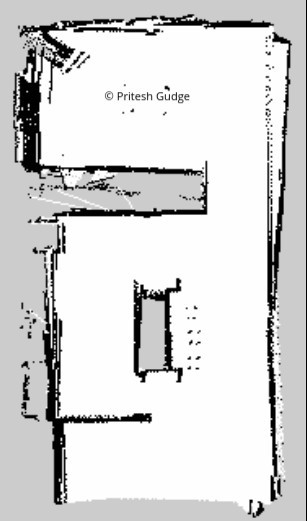
\includegraphics[width=\linewidth]{images/kitchen2dmap}
      \caption{Kitchen World 2D map}
      \label{fig:kitchen2d}
\end{figure}


\begin{figure}[thpb]
      \centering
      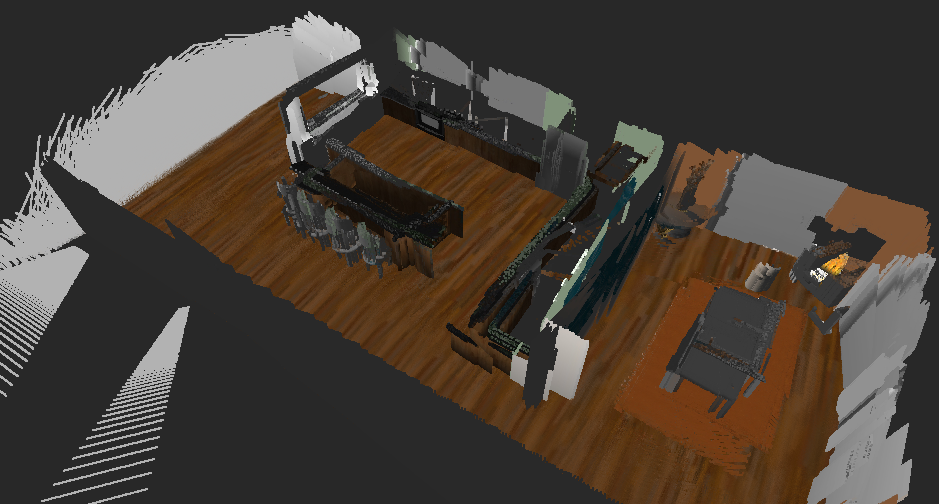
\includegraphics[width=\linewidth]{images/3dmap2}
      \caption{Kitchen World 3D Map}
      \label{fig:kitchen3d}
\end{figure}

\subsection{Custom Cafe World}

\subsection{Technical Comparison} % only facts
The kitchen\_dining model performed significantly better then the student created cafe model. This was due to the richer and more complex features of the kitchen\_dining model.

\section{Discussion}
The robot was teleoped (navigated via the keyboard) around the room. At some points the robot did not move forward. This appeared to be when it started to perform loop closure. 

However the 3D map quickly started to resemble the physical kitchen dining gazebo model. To improve loop detection rates some, on the spot circles were performed. Of particular note were the features in the main kitchen area. More SURF features were identified there as there was more variation in the surface s.

............
Kp/MaxFeatures was halved to 200 and Vis/MinInliers was reduced from 15 to 10.
...........

.......The nick building gazebo model wall surfaces were tiled, repeatable pattern with lack of other discerning features sometimes caused the loop closure detection to map to an incorrect previous image. This then distorted the map. Additional features were added to achieve a successful map............



\section{Conclusion / Future work}

Mapping is important to help understand the world. There are a plethora of sensors and of interest is the about to arrive solid state lidars. As the price point of these sensors continues to drop it will open up opportunities to create richer and more realistic 3D maps at a cheaper price point.
Being able to map an environment cost effectively to create a replicated virtual world will increasingly be important to allow for the training of deep learning models. We are actively looking to do this and then supplant the trained model back into a robot so it can navigate in the original environment that was mapped.

\subsection{Modifications for Improvement}
Examples:
\begin{itemize}
\item Adding more sensors to collect data e.g. 3D Lidar
\item Modifying the sensor location and layout. e.g. Adding RGBD camera's to the sides of the robot, to collect data about the side surrounding
\end{itemize}

\subsection{Hardware Deployment}
\begin{enumerate}
\item To be deployed on hardware, a computation unit and appropriate sensors will have to be installed on the robot chassis and the wheels. Proper calibration and verification needs to be done to limit the errors.
\item High CPU and RAM hardware is required to perform SLAM data collection from the multiple sensors, especially to detect loop closures online.
\end{enumerate}



\bibliography{bib}
\bibliographystyle{ieeetr}

\end{document}